\documentclass[11pt]{report}
\usepackage[english, german]{babel}
\usepackage{geometry}                % See geometry.pdf to learn the layout options. There are lots.
\geometry{a4paper}                   % ... or a4paper or a5paper or ... 
%\usepackage[parfill]{parskip}    % Activate to begin paragraphs with an empty line rather than an indent
\usepackage{xifthen}
\usepackage{xstring}			% to check content of strings in xifthen
\usepackage{graphicx}
\usepackage[usenames,dvipsnames,table]{xcolor}
\usepackage{amssymb}
\usepackage{epstopdf}
\usepackage[utf8]{inputenc}
\usepackage{hyperref}
\usepackage{fancyhdr}
%\usepackage{natbib}
\usepackage{url}

\newcommand{\titleofthesis}{AKKalytics}
\newcommand{\department}{Informatik} % Replace by your department

\newcommand{\firstauthor}{Felix Kronsteinerr}
\newcommand{\firstauthorclass}{5AHIF}
\newcommand{\secondauthor}{Adzamija Alen}
\newcommand{\secondauthorclass}{5AHIF}
\newcommand{\thirdauthor}{Klatzer Emanuel}
\newcommand{\thirdauthorclass}{5AHIF}

\newcommand{\duedateen}{April 4, 2018} % due date in english format
\newcommand{\duedatede}{4. April 2018} % due date in german format
\newcommand{\supervisor}{Gerhard Aistleitner}
\newcommand{\projectpartner}{MIC}
 % Set basic data (author, title, etc.) of your thesis
\IfStrEq*{\languagename}{english}
	{
		\newcommand{\dalabel}{Diploma Thesis}
		\newcommand{\submittedlabel}{Submitted by}
		\newcommand{\datelabel}{Date}
		\newcommand{\duedatevalue}{\duedateen}
		\newcommand{\supervisorlabel}{Supervisor}
		\newcommand{\projectpartnerlabel}{Project Partner}
	}
	{
		\newcommand{\dalabel}{Diplomarbeit}
		\newcommand{\submittedlabel}{Eingereicht von}
		\newcommand{\datelabel}{Datum}
		\newcommand{\duedatevalue}{\duedatede}
		\newcommand{\supervisorlabel}{Betreuer}
		\newcommand{\projectpartnerlabel}{Projektpartner}
	}
 % This file should not really be touched

\begin{document}
\rhead{
\includegraphics[scale=.9]{images/Logo.png}}
\cfoot{}
\begin{titlepage}
\thispagestyle{fancy}

\begin{center}

\vspace*{8em}

{\LARGE \dalabel}

\vspace{2em}

{\large Höhere Technische Bundeslehranstalt Leonding \\[.5em]
Abteilung für \department}

%\vspace{8em}
\vspace*{\fill}

{\Huge \titleofthesis}
\end{center}

%\vspace{8em}
\vspace*{\fill}

\begin{tabular}{ll}
\ifthenelse{\isundefined{\firstauthor}}{}{\submittedlabel: & {\bf \firstauthor, \firstauthorclass}}
\ifthenelse{\isundefined{\secondauthor}}{}{ \\[.5em] & {\bf \secondauthor, \secondauthorclass}}
\ifthenelse{\isundefined{\thirdauthor}}{}{ \\[.5em] & {\bf \thirdauthor, \thirdauthorclass}}
\ifthenelse{\isundefined{\fourthauthor}}{}{ \\[.5em] & {\bf \fourthauthor, \fourthauthorclass}}
 \\[.5em]
\datelabel: & {\bf \duedatevalue} \\[.5em]

\supervisorlabel: & {\bf \supervisor} \\[.5em]

\ifthenelse{\isundefined{\projectpartner}}{}{\projectpartnerlabel: & {\bf \projectpartner}}
\end{tabular}
\end{titlepage}
 % Should not be necessary to touch this file
\section*{Declaration of Academic Honesty}
Hereby, I declare that I have composed the presented paper independently on my own and without any other resources than the ones indicated. All thoughts taken directly or indirectly from external sources are properly denoted as such.

This paper has neither been previously submitted to another authority nor has it been published yet. \\[1em]
Leonding, \duedateen \\[5em]
\ifthenelse{\isundefined{\firstauthor}}{}{\firstauthor}
\ifthenelse{\isundefined{\secondauthor}}{}{\kern-1ex, \secondauthor}
\ifthenelse{\isundefined{\thirdauthor}}{}{\kern-1ex, \thirdauthor}
\ifthenelse{\isundefined{\fourthauthor}}{}{\kern-1ex, \fourthauthor} \\[5em]

\begin{otherlanguage}{german}
\section*{Eidesstattliche Erklärung}
Hiermit erkläre ich an Eides statt, dass ich die vorgelegte Diplomarbeit selbstständig und ohne Benutzung anderer als der angegebenen Hilfsmittel angefertigt habe. Gedanken, die aus fremden Quellen direkt oder indirekt übernommen wurden, sind als solche gekennzeichnet.

Die Arbeit wurde bisher in gleicher oder ähnlicher Weise keiner anderen Prüfungsbehörde vorgelegt und auch noch nicht veröffentlicht. \\[1em]
Leonding, am \duedatede \\[5em]
\ifthenelse{\isundefined{\firstauthor}}{}{\firstauthor}
\ifthenelse{\isundefined{\secondauthor}}{}{\kern-1ex, \secondauthor}
\ifthenelse{\isundefined{\thirdauthor}}{}{\kern-1ex, \thirdauthor}
\ifthenelse{\isundefined{\fourthauthor}}{}{\kern-1ex, \fourthauthor} \\[5em]
\end{otherlanguage}

\begin{abstract}
Here it is described what the thesis is all about. The abstract shall be brief and concise and its size  shall not go beyond one page. Furthermore it has no chapters, sections etc. Paragraphs can be used to structure the abstract. If necessary one can also use bullet point lists but care must be taken that also in this part of the text full sentences and a clearly readable structure are required.

Concerning the content the following points shall be covered. 

\begin{enumerate}
	\item {\em Definition of the project:} What do we currently know about the topic or on which results can the work be based? What is the goal of the project? Who can use the results of the project?
	
	\item {\em Implementation:} What are the tools and methods used to implement the project?
	
	\item {\em Results:} What is the final result of the project?
\end{enumerate}
This list does not mean that the abstract must strictly follow this structure. Rather it should be understood in that way that these points shall be described such that the reader is animated  to dig further into the thesis.

Finally it is required to add a representative image which describes your project best. The image here shows Leslie Lamport the inventor of \LaTeX.

\begin{flushright}
	\includegraphics[scale=.25]{images/leslie_lamport.jpg}
\end{flushright}

\end{abstract}

\begin{otherlanguage}{german}
\begin{abstract}
An dieser Stelle wird beschrieben, worum es in der Diplomarbeit geht. Die Zusammenfassung soll kurz und prägnant sein und den Umfang einer Seite nicht übersteigen. Weiters ist zu beachten, dass hier keine Kapitel oder Abschnitte zur Strukturierung verwendet werden. Die Verwendung von Absätzen ist zulässig. Wenn notwendig, können auch Aufzählungslisten verwendet werden. Dabei ist aber zu beachten, dass auch in der Zusammenfassung vollständige Sätze gefordert sind.

Bezüglich des Inhalts sollen folgende Punkte in der Zusammenfassung vorkommen: 

\begin{itemize}
	\item {\em Aufgabenstellung:} Von welchem Wissenstand kann man im Umfeld der Aufgabenstellung ausgehen? Was ist das Ziel des Projekts? Wer kann die Ergebnisse der Arbeit benutzen?
	
	\item {\em Umsetzung:} Welche fachtheoretischen oder -praktischen Methoden wurden bei der Umsetzung verwendet?
	
	\item {\em Ergebnisse:} Was ist das endgültige Ergebnis der Arbeit?
\end{itemize}
Diese Liste soll als Sammlung von inhaltlichen Punkten für die Zusammenfassung verstanden werden. Die konkrete Gliederung und Reihung der Punkte ist den Autoren überlassen. Zu beachten ist, dass der/die LeserIn beim Lesen dieses Teils Lust bekommt, diese Arbeit weiter zu lesen.

Abschließend soll die Zusammenfassung noch ein Foto zeigen, das das beschriebene Projekt am besten repräsentiert. Das folgende Bild zeigt Leslie Lamport, den Erfinder von \LaTeX.

\begin{flushright}
	\includegraphics[scale=.25]{images/leslie_lamport.jpg}
\end{flushright}

\end{abstract}
\end{otherlanguage}

\section*{Acknowledgments}
If you feel like saying thanks to your grandma and/or other relatives.
 % Declaration of Academic Honesty, Abstracts, Acknowledgments, 

\tableofcontents

\chapter{Introduction}
\section{Initial Situation}
Common word processors do not prepare print-like documents in so far as these programs do not reflect the rules of professional printing which have been grown over centuries. These rules contain clear requirements for balancing page layouts, the amount of white space on pages, font-handling, etc. Donald Knuth's TeX package (see~\cite{knuth_texbook_1984}) is a word processor which conforms to these printing rules. This package was enhanced by Leslie Lamport by providing more text structuring commands. He called his package LaTeX~\cite{lamport_latex_1985}.

When preparing a thesis, we want not only to have our content on a top level, we also want to commit to a high level of formal criteria. Therefore, we request our students to use one of these professional printing production environments like TeX or LaTeX.

Furthermore students should train their scientific writing skills. This includes a clear and structured break-down of their ideas, a high-level and clear wording, and the training of transparent citations of ideas from other sources than from theirs. A good source for more information concerning technical and scientific writing can be found in~\cite{rechenberg_technisches_2006}.

\section{Goals}
The general goals and objectives of the project are described here. Care must be taken that the goals documented here are purely project goals and have nothing to do with individual goals of the team members. If individual goals should be part of the thesis they are listed in appendix~\ref{cha:individual-goals}.

\section{Overview}
Details of the diploma thesis have to be aligned between student and supervisor. This should be a basic structure to facilitate the first steps when students start to write their theses.

Never forget to add some illustrative images. Images must not be messed up with your normal text. They are encapsulated in floating bodies and referenced in your text. An example can be seen in figure~\ref{fig:sample}. As you can see, figures are placed by default on top of the page nearby the place where they are referenced the first time. Furthermore you can see that a list of figures is maintained automatically which can be included easily by typing the command \verb1\listoffigures1 into your document.

\begin{figure}
\begin{center}
	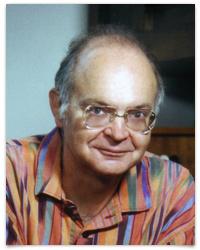
\includegraphics[scale=.5]{images/don_knuth.jpg}
\end{center}
	\caption{Don Knuth, the inventor of \TeX}
	\label{fig:sample}
\end{figure}

\section{Basic Terminology}
As usual the very basic terminology is briefly explained here. Most probably the explanations here only scratch a surface level. More detailed explanations of terminology goes into chapter~\ref{cha:theoretical-background}.

\section{Related Work and Projects}
Here a survey of other work in and around the area of the thesis is given. The reader shall see that the authors of the thesis know their field well and understand the developments there. Furthermore here is a good place to show what relevance the thesis in its field has.

\section{Structure of the Thesis}
%dsflkjas flaksjfl asdfj as lfjldsajflaksdjf sa dfjlasdkfj sadlfjasdklf als dfj l dfsdfsdfn chapter~\ref{cha:used-technologies} (\nameref{cha:used-technologies}) on page~\pageref{cha:used-technologies} we describe the used technologies.
Finally the reader is given a brief description what (s)he can expect in the thesis. Each chapter is introduced with a paragraph roughly describing its content.
\chapter{Theoretical Background}\label{cha:theoretical-background}
The details of the structure of your thesis have to be aligned with the supervising teacher. However, most of the theses require to have some description of the models used or some other theoretical background necessary to understand the rest of the text.

Since there is enough space here a table is added to show the basic usage of tables in a scientific document. Similarly to images these are also kept outside the normal text flow in a so-called floating body. Table~\ref{tab:types-of-floating-bodies} shows different options \cite{khason_computer_2008, krasner_description_1988}.

\begin{table}
	\begin{center}
	\begin{tabular}{|l|l|}
		\hline
		\cellcolor{Gray}\textcolor{White}{Body type} & \cellcolor{Gray}\textcolor{White}{Floats} \\
		\hline
		Image & Always \\
		\hline
		Table & Always \\
		\hline
		Algorithm & Sometimes \\
		\hline
	\end{tabular}
	\end{center}
	\caption{Different types of floating bodies}
	\label{tab:types-of-floating-bodies}
\end{table}
\chapter{Aufgabenstellung}\label{cha:used-technologies}

\chapter{BlaBlö}
\section{HahAlenGay}
Jo des ghert so
\chapter{Architektur}
\chapter{Datenquellen und Ihr Aufbau}
\chapter{Extract}
\chapter{Transform}
\chapter{Load}
\chapter{Visualisierung}
\section{Kapitel1}
\section{Kapitel2}
\section{Kapitel3}
\section{Kapitel4}
\chapter{Die Arbeitsumgebung}
\section{AWS}
\section{Linux}
\section{Portainer}
\section{IntelliJ}
\section{Vim}
\section{Docker}
\chapter{Verwendete Technologien}
\section{Kapitel1}
\section{Kapitel2}
\section{Kapitel3}
\section{Kapitel4}
\chapter{Databus}
\chapter{Kotlin}
\chapter{Gradle}
\chapter{Kafka}
\chapter{Portainer}
\chapter{Load}
\chapter{NO SQL}
\chapter{Python}
\chapter{Spark}
\chapter{Was sind Visualisierungs Applikationen (FK)}
Visualisierungs Applikationen sind eine Möglichkeit Daten als Grafiken widerzuspiegeln. Die Daten können auf vielfältige Art und weise zusammengestellt werden. Nicht jede Visualisierungs Applikation kann dieselben Datenquellen benutzen und verarbeiten. In Microsoft Word kann man zum Beispiel ausschließlich Microsoft Excel Tabellen für die Diagramme einfügen. In Spezialisierteren Applikationen können weitaus mehr Datenquellen verwendet werden wie Daten direkt aus einer Datenbank auslesen oder mit einer REST Schnittstelle von einem Server zu bekommen.
\section{Warum Visualisierungs tools}
Viele Unternehmen sammeln täglich riesige Mengen an Daten über ihre Kunden, Mitarbeiter, den Markt und viele andere Dinge, aber dieses Wissen ist einzeln betrachtet in bedeutungslosen Zahlen versteckt. Kombiniert man aber diese Daten könnten sie analysiert und visualisiert werden, um benutzerfreundliche und verständliche Diagramme zu erstellen, die helfen können, Marktveränderungen vorherzusagen oder den Gewinn durch intelligente Kostenreduzierung zu erhöhen. 
Dies könnte entweder von einem Betreiber genutzt werden, der ansprechende Diagramme für seine Präsentationen und Berichte verwendet, oder von Datenanalysten, die diese Diagramme studieren und nützliche Informationen ableiten, um Fragen zu beantworten wie "Warum steigt der Markt in Großbritannien, obwohl es den Brexit gibt, und wie können wir das, was in dieser Region funktioniert, in andere Regionen bringen?

\chapter{Was sind Visualisierungs Applikationen}
\section{Kapitel1}
\section{Kapitel2}
\section{Kapitel3}
\section{Kapitel4}
\chapter{Der Visualisierungsprozess}
\section{Einrichten von AWS}
\section{Installierung von Elasticsearch und Kibana}
\section{Die REST-API Schnittstelle von Elasticsearch}
\section{Die Erstellung von Grafiken mit Kibana}
\section{Probleme beim Visualisierungsprozess}
\chapter{Summary}
Here you give a summary of your results and experiences. You can add also some design alternatives you considered, but kicked out later. Furthermore you might have some ideas how to drive the work you accomplished in further directions.





\bibliography{da_bibliography,FK_Zotero_Bibliothek}{}
\bibliographystyle{alphaurl} % alternatives plainurl, alphaurl;  german alternative: dinat (but add package natbib)

\listoffigures
\listoftables
\chapter*{Project Log Book}
\begin{tabular}{|l|l|l|l|}
\hline
Date & Participants & Todos & Due\\
\hline
\end{tabular}

\appendix
\chapter{Additional Information} \label{cha:additional-information}
If needed the appendix is the place where additional information concerning your thesis goes. Examples could be:
\begin{itemize}
	\item Source Code
	\item Test Protocols
	\item Project Proposal
	\item Project Plan
	\item Individual Goals
	\item \ldots
\end{itemize}
Again this has to be aligned with the supervisor.
\chapter{Individual Goals} \label{cha:individual-goals}
This is just another example to show what content could go into the appendix.
\end{document}  